\section{Die Genauigkeitsmessung des Extraktionsalgorithmus}
\label{sec:evaluierung}

Der entwickelte Algorithmus deckt die grundlegenden Elementtypen für die Datenextraktion ab.
Wie bereits eingangs erwähnt wurde, ist die Qualität der Extraktion von großer Bedeutung - doch wie genau ist der
entwickelte Algorithmus?
Genau diese Frage wird in diesem Kapitel beantwortet, um eine grobe Aussage für das weitere Matchingverfahren zu
treffen.

\subsection{Die Testdaten der Evaluierung}
\label{subsec:testdaten}
Sowohl für das Antrainieren der Extraktionsregeln als auch für die Evaluierung der Ergebnisse wurden die von idealo
zur Verfügung gestellten Angebotsdaten verwendet.
Für die nachfolgenden Messungen wurden 7500 Angebote von 50 Shops genutzt.

Je Händler wurden max.\ 50 Angebote als Trainingsmenge für die Erstellung der Regeln und 100 Angebote als Testmenge für
die Evaluierung verwendet.
Die Auswahl der Shops erfolgte basierend auf den ersten Listeneinträgen der Shopübersicht\footnotemark von idealo.
\footnotetext{https://www.idealo.de/preisvergleich/AllePartner.html}

Alle nachfolgenden Messungen basieren auf einem Schnappschuss der Angebotsdaten inklusive der verlinkten Webseiten.
Die Links wurden nicht durch die URL-Cleaner-Komponente bereinigt, da sonst die Angebotsdaten von idealo
möglicherweise nicht mit denen von der Webseite übereinstimmen.
Damit die Trackingstatistiken der Shopbetreiber nicht verfälscht werden, wurden nicht mehr als 150 Angebote je Shop
heruntergeladen.

Eine Analyse der gesamten Testdaten hat ergeben, dass für jedes Angebot die Angaben zum Titel, dem Preis und der SKU
existieren.
Am seltensten existieren hingegen die HAN (68\%) und die Produktbeschreibung (77\%) eines Angebots.

Das Verhältnis der fehlenden zu den vorhandenen Produktattributen der Trainingsmenge ähnelt dem Verhältnis der
Testmenge und weicht um maximal 0.88\% bei der Produkteigenschaft "Marke" ab.

\subsection{Die Messergebnisse}
\label{subsec:genauigkeitsmessung}
Die Genauigkeit des Parser wurde bestimmt, indem die Extraktionsregeln auf der Testmenge angewandt wurden.
Die Treffergenauigkeit wurde dabei in Abhängigkeit der Menge der Angebote \textit{SaS}, welche für das Anlernen
verwendet wurden, sowie des in Kapitel~\ref{subsec:bewertungssystem} eingeführten Filter-Schwellwertes \textit{F}
bestimmt.
In der Tabelle~\ref{tab:accuracy-precision} sind die Treffergenauigkeit (\textit{accuracy}) und die Genauigkeit
(\textit{precision}) aufgeführt.
Die Treffergenauigkeit gibt an, wie oft ein Produktattribut korrekt erfasst wurde und entspricht in diesem Fall der
Trefferquote (\textit{recall}).
Die Genauigkeit berücksichtigt zusätzlich die Fälle, in denen der Parser explizit nichts zurück gibt.
In allen Statistiken wurden die Produkteigenschaften ignoriert, bei denen idealo keine Produktattribute gespeichert hat.
In diesem Fall ist es nicht möglich zu entscheiden, ob das vom Parser extrahierte korrekt ist.

\begin{table}[h]
    \centering
    \begin{tabular}{ c | c c c | c c c }
        &   \multicolumn{3}{c}{\textit{Treffergenauigkeit in \%}}    &   \multicolumn{3}{c}{\textit{Genauigkeit in \%}} \\
        \textbf{F\textbackslash SaS} & \textbf{10} & \textbf{20} & \textbf{50} & \textbf{10} & \textbf{20} & \textbf{50}  \\
        \hline
        \textbf{0}       &   50.59 &   50.78 &   51.07         &   72.73 &   70.81 &   69.62 \\
        \textbf{0.5}     &   52.12 &   53.50 &   \textbf{53.98}&   88.66 &   90.39 &   91.22 \\
        \textbf{0.6}     &   51.87 &   53.07 &   53.15         &   94.15 &   94.03 &   94.93 \\
        \textbf{0.7}     &   50.15 &   51.37 &   52.02         &   96.15 &   96.39 &   95.86 \\
        \textbf{0.8}     &   47.92 &   49.69 &   50.05         &   97.84 &   97.81 &   97.76 \\
        \textbf{0.9}     &   44.61 &   46.92 &   46.57         &   98.16 &   98.14 &   98.42 \\
        \textbf{1.0}     &   41.48 &   39.27 &   36.00         &   98.17 &   97.64 &   \textbf{98.90}

    \end{tabular}
    \caption{Treffergenauigkeit und Genauigkeit bei unterschiedlichen Konfigurationen}
    \label{tab:accuracy-precision}
\end{table}

Die vom Parser extrahierten Angebotsinformationen werden von der Matcher-Komponente für den ähnlichkeitsbasierten
Vergleich verwendet.
Dazu ist es wichtig, eine gute Balance zwischen Treffergenauigkeit und Genauigkeit zu finden.
Da es nicht unbedingt darum geht, dass die extahierten Informationen \textit{exakt} dem Schema von idealo entspricht,
ist die Treffergenauigkeit etwas wichtiger, als die Genauigkeit.
Laut den in Tabelle~\ref{tab:accuracy-precision} angegeben Werten, scheinen die besten Ergebnisse bei einem
Schwellwert von $F=0.6$ und $SaS=50$ erreicht zu werden.

Für jede Nichtübereinstimmung wurde die Levenshtein-Distanz zum erwarteten Wert von idealo berechnet.
In etwa 50\% der Nichtübereinstimmungen haben eine Distanz kleiner gleich drei und sind somit sehr ähnlich.
Eine manuelle Prüfung hat ergeben, dass oftmals Kodierungsfehler oder unterschiedliche Trennzeichen eine eindeutige
Übereinstimmung verhindern.

Eine nähere Betrachtung der Kennziffern je Attribut liefert weitere Aufschlüsse, welche für das Matching relevant sind.

\begin{figure}[H]
    \centering
    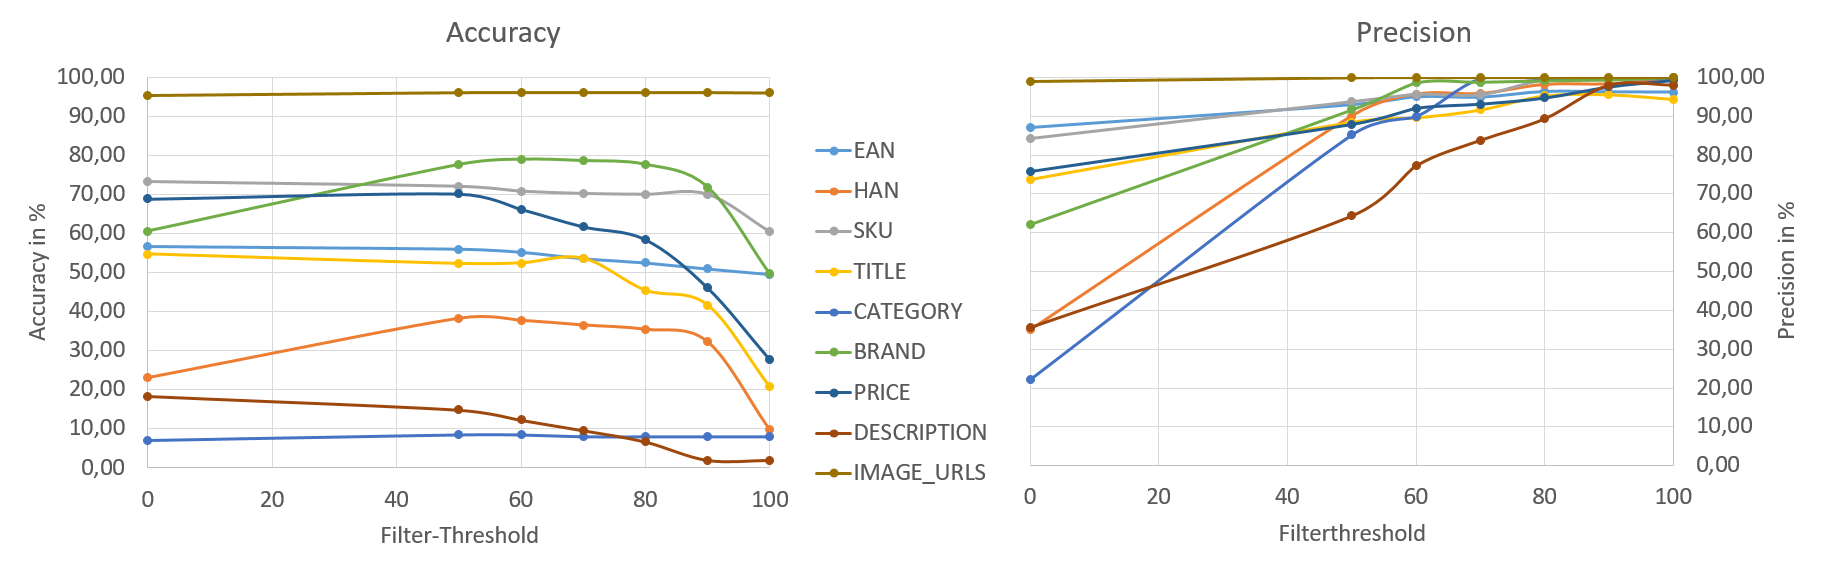
\includegraphics[width=\textwidth]{resources/accuracy-and-precision-per-attribute.PNG}
    \caption{Treffergenauigkeit und Genauigkeit pro Attribut für $SaS=50$}
    \label{abb:testdaten}
\end{figure}

Den Diagrammen aus Abbildung~\ref{abb:testdaten} kann man mehrere, für das Matching nützliche Informationen entnehmen.
Wie erwartet, wird die Produktbeschreibung und die Kategorie selten extrahiert.
Dies hängt damit zusammen, dass diese Informationen am stärksten von idealo manipuliert werden.
Interessanterweise wird die HAN ebenfalls selten extrahiert, was vermutlich mit den Testdaten zusammenhängt.
In diesen kommt die HAN nur in zwei von drei Angeboten vor und ist damit die am seltensten angegebene
Produkteigenschaft.
Am häufigsten wird die Bildurl und die Marke gefunden.
Aus dem Diagramm, welches die Genauigkeit je Attribut darstellt kann man sehr gut entnehmen, dass der Schwellwert ein
gutes Mittel ist, die Genauigkeit direkt zu beeinflussen.
Insgesamt kann man für die Matcher-Komponente eine sehr interessante Erkenntnis gewinnen, welche wir vorher nicht in
Betracht gezogen haben.
So scheint die Bildurl sehr häufig und korrekt erfasst zu werden.
Die Bildurl kann als starker Selektor, ähnlich wie den eindeutigen Produkteigenschaften verwendet werden.

\subsection{Mögliche Fehlerquellen der Messung}
\label{subsec:fehlerquellen}

Es musste leider festgestellt werden, dass beim Erstellen der Evaluierungsdaten ein Shop durch eine
Captcha-Absicherung keine nutzbaren Webseiten lieferte.
Für diesen Shop konnten folglich keinerlei Regeln für keine der Produkteigenschaften erstellt werden.
Dies wirkt sich leicht negativ auf die Treffergenauigkeit aus.

Des Weiteren hat die Verwendung der idealo-Daten als Trainings- und Lerndaten den Nachteil, dass diese teilweise
manuell oder durch Normalisierungsprozesse von idealo manipuliert wurden.
Die Angebotsdaten können somit von den Spezifikationen der Webseite abweichen.
Dieser Fall wurde sehr häufig bei dem Titel und der Produktbeschreibung beobachtet.
Dies führt dazu, dass die Erstellung der Regeln erschwert wird und manche eigentlich korrekt extrahierte
Produktattribute fälschlicherweise als inkorrekt markiert werden.